%\documentclass{beamer}
\documentclass[aspectratio=169]{beamer}
\usetheme{Boadilla}

%\usetheme{Warsaw}
%\setbeamercovered{transparent}
\beamertemplatetransparentcoveredhigh
\usepackage[portuges]{babel}
\usepackage[latin1]{inputenc}
\usepackage{lmodern}
\usepackage[T1]{fontenc}
\usepackage{hyperref} 
\usepackage[portuguese, linesnumbered, vlined, titlenumbered, ruled]{algorithm2e}

\newcommand{\eng}[1]{\textsl{#1}}
\newcommand{\cod}[1]{\texttt{#1}}

\title[Apresenta��o]{Curso Intelig�ncia Artificial: do Zero ao Infinito}
\author[Frederico Oliveira]{Modelos em Produc�o}
\institute[UFMT]{Universidade Federal de Mato Grosso}
\date{}
%\titlegraphic{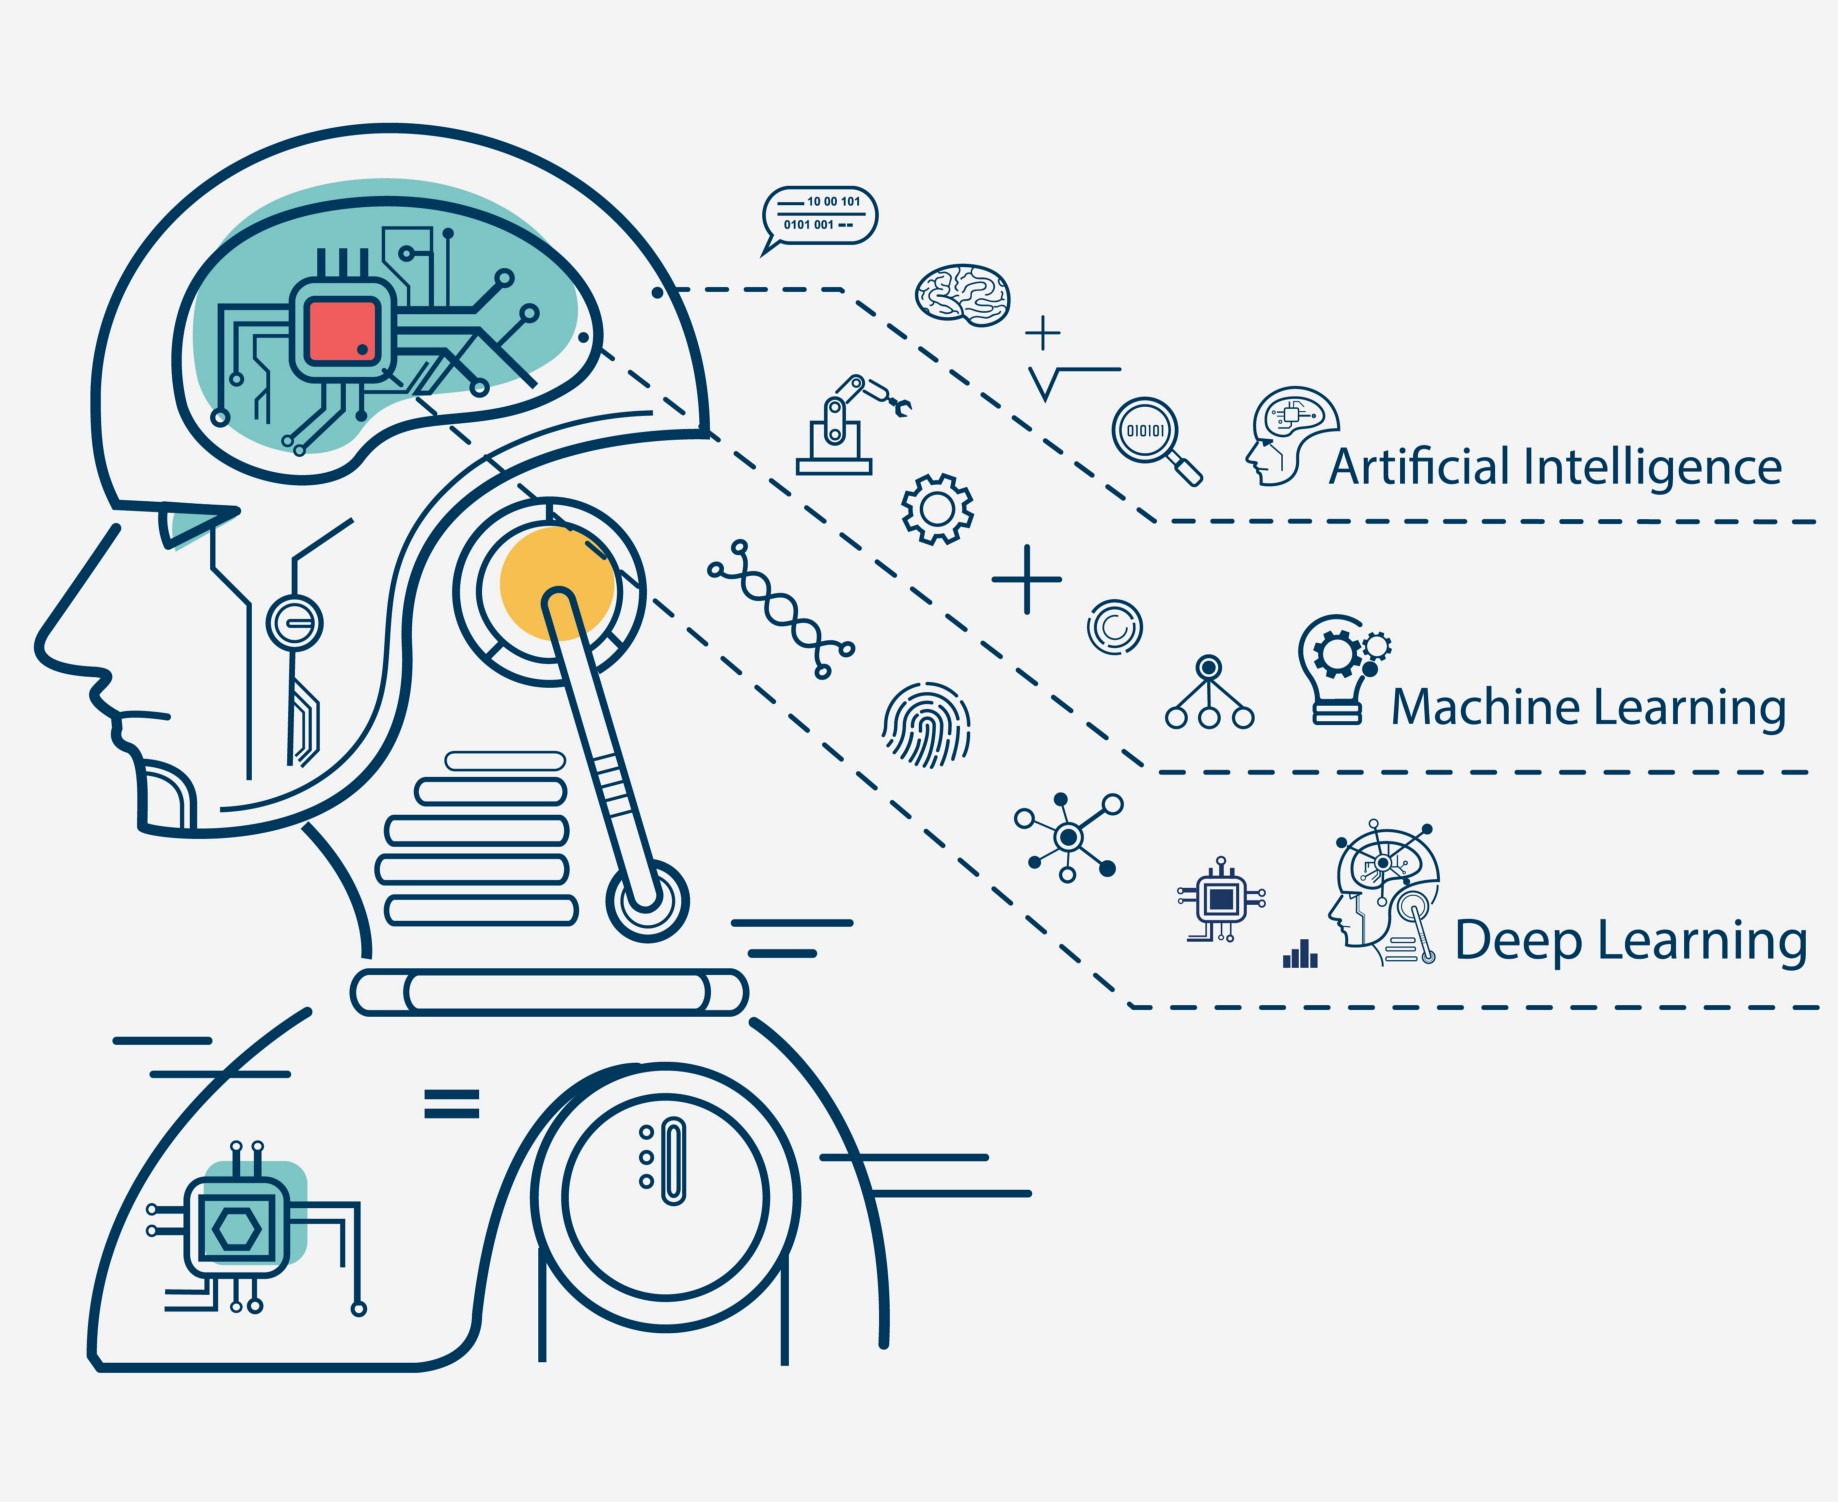
\includegraphics[width=\textwidth,height=.5\textheight]{imgs/intro.jpeg}}
%\usebackgroundtemplate{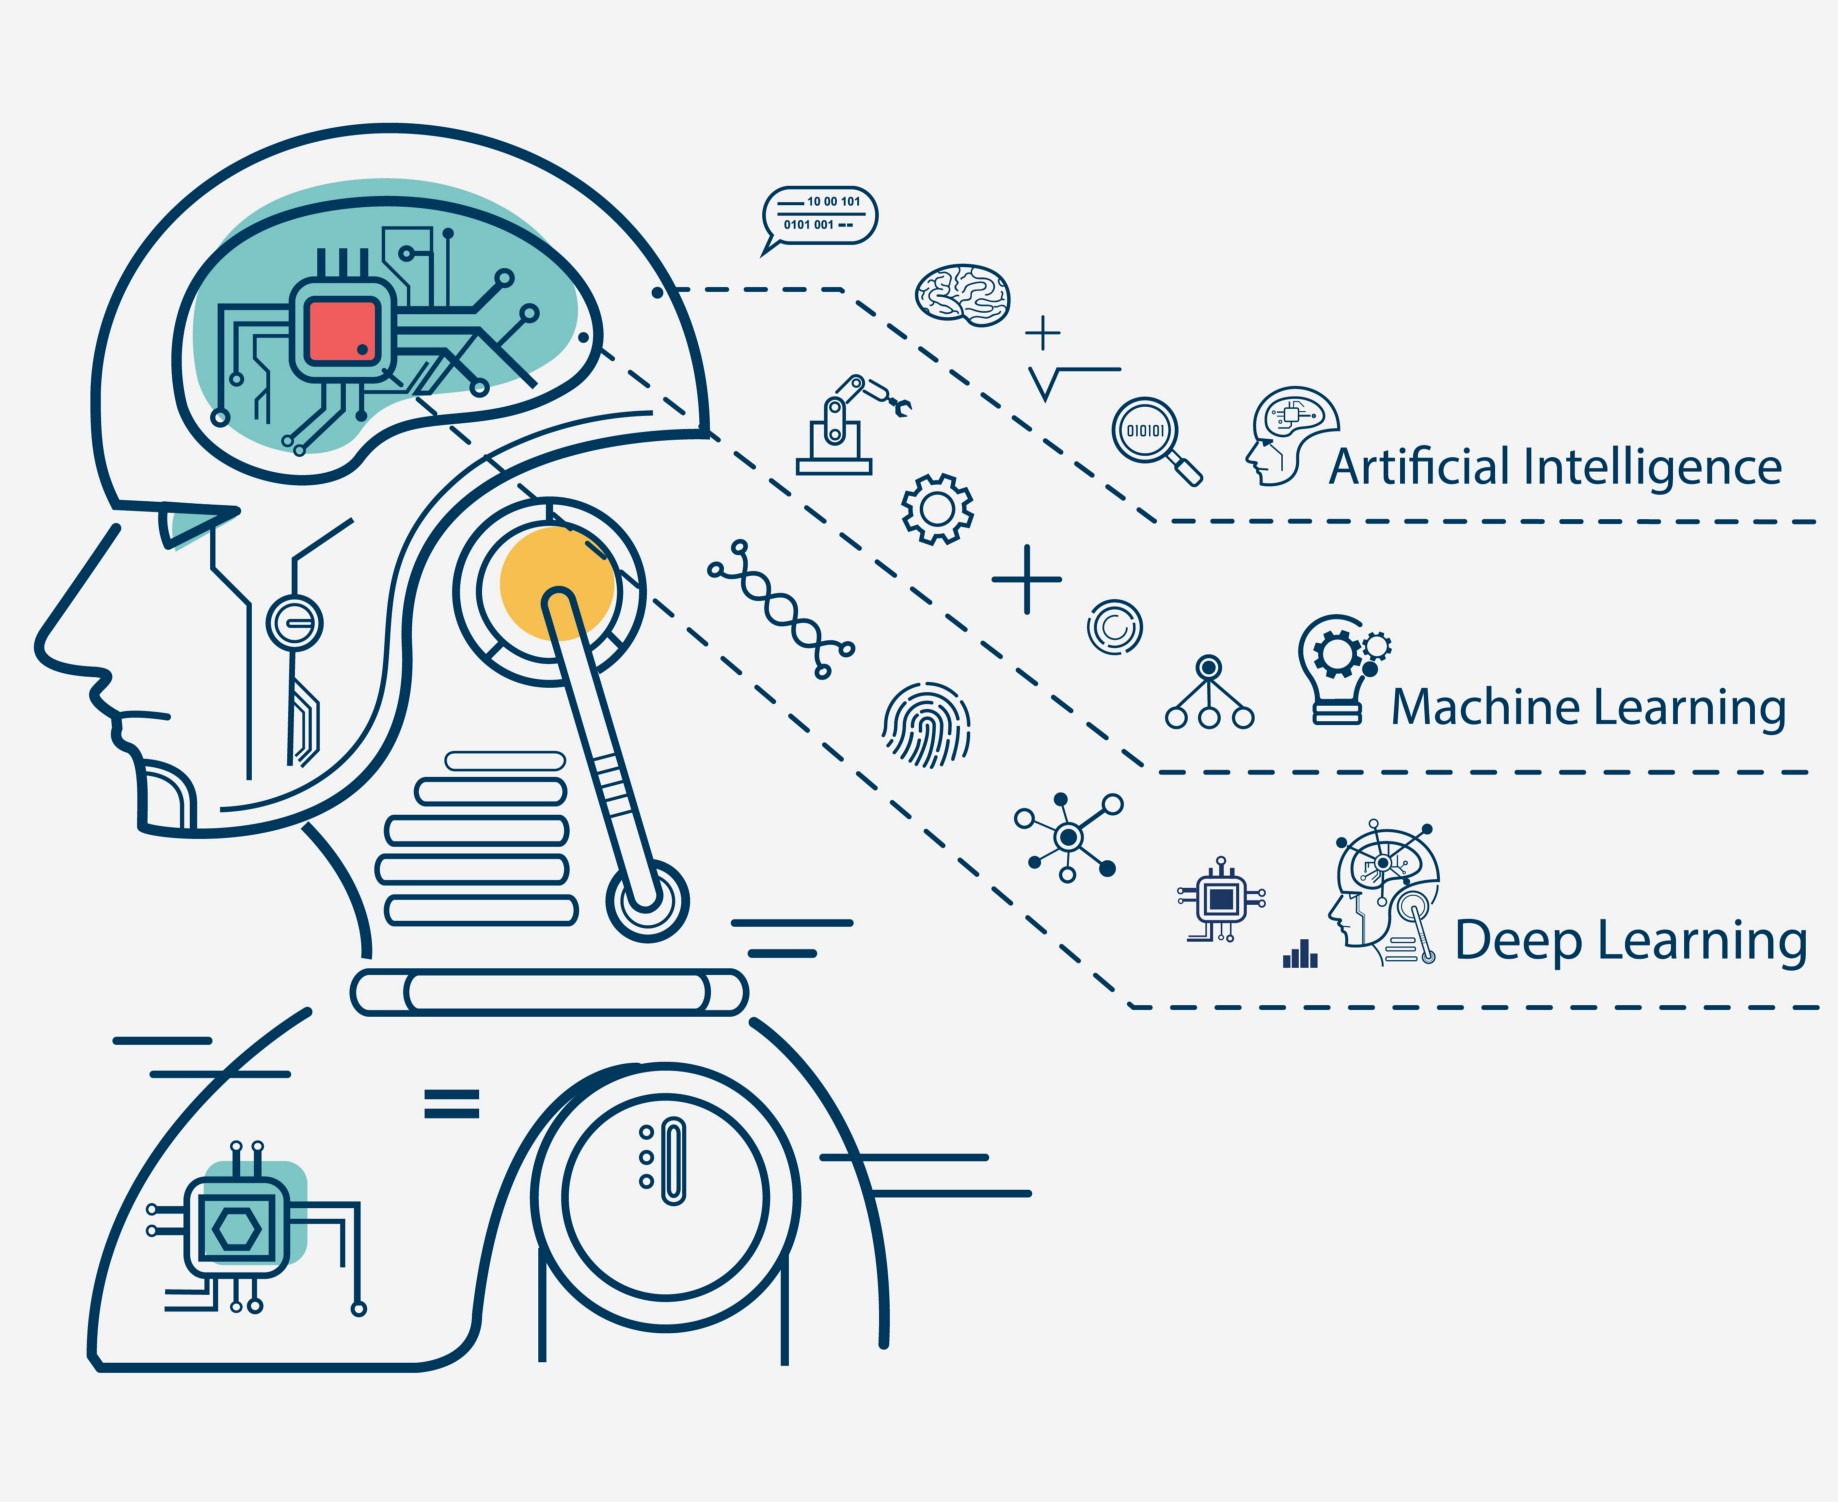
\includegraphics[width=\paperwidth]{imgs/intro.jpeg}}
\begin{document}

\begin{frame}[plain]
  \titlepage
\end{frame}

%%%%%%%%%%%%%%%%%%%%%%%%%%%%%%%%%%%%%%%%%%%%%%%%%%%%%%%%%%%%%%%%%%%%%%%%%%%%%%%%%%%%%%%%%%%%%%%%%%%%%%%%%%%%%%%%
%\section*{Roteiro}
%%%%%%%%%%%%%%%%%%%%%%%%%%%%%%%%%%%%%%%%%%%%%%%%%%%%%%%%%%%%%%%%%%%%%%%%%%%%%%%%%%%%%%%%%%%%%%%%%%%%%%%%%%%%%%%%

\begin{frame}
  \frametitle{Agenda}
  \tableofcontents
\end{frame}



%%%%%%%%%%%%%%%%%%%%%%%%%%%%%%%%%%%%%%%%%%%%%%%%%%%%%%%%%%%%%%%%%%%%%%%%%%%%%%%%%%%%%%%%%%%%%%%%%%%%%%%%%%%%%%%%%
\section{TF Serving}
%%%%%%%%%%%%%%%%%%%%%%%%%%%%%%%%%%%%%%%%%%%%%%%%%%%%%%%%%%%%%%%%%%%%%%%%%%%%%%%%%%%%%%%%%%%%%%%%%%%%%%%%%%%%%%%%

\begin{frame}{TF Serving}
\begin{itemize}
\item Podemos disponibilizar um modelo para Object Detection utilizando o framework  {\bf TF Serving}.
\item TF Serving � um sistema de servi�o flex�vel e de alto desempenho para modelos de aprendizado de m�quina, projetado para ambientes de produ��o. 
\item Facilita a implanta��o de novos algoritmos e fornece integra��o imediata com os modelos do TensorFlow.
\end{itemize}

\vspace{1cm}
\tiny{Fonte: \href{https://www.tensorflow.org/tfx/guide/serving}{Documenta��o Oficial Tensorflow}}
\end{frame}

%%%%%%%%%%%%%%%%%%%%%%%%%%%%%%%%%%%%%%%%%%%%%%%%%%%%%%%%%%%%%%%%%%%%%%%%%%%%%%%%%%%%%%%%%%%%%%%%%%%%%%%%%%%%%%%%%

\begin{frame}{TF Serving}
\begin{figure}[h]
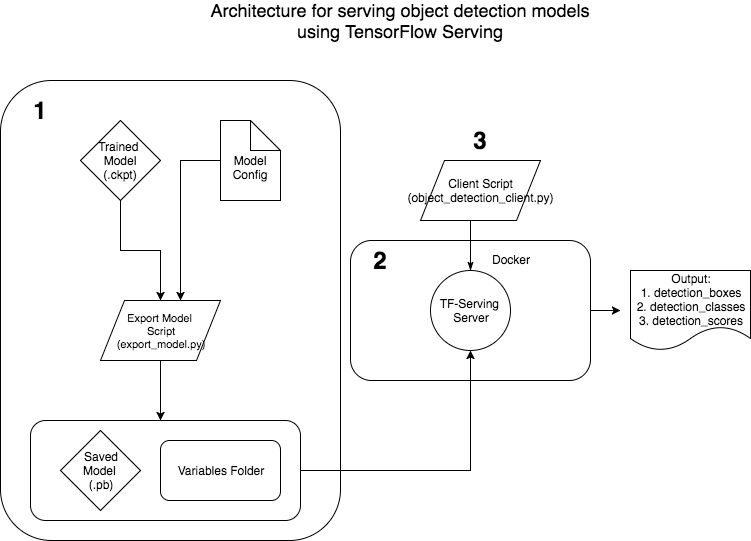
\includegraphics[width=10cm]{imgs/tf_serving_architecture.png}
\end{figure}

\vspace{1cm}
\tiny{Fonte: \href{https://www.freecodecamp.org/news/how-to-deploy-an-object-detection-model-with-tensorflow-serving-d6436e65d1d9/}{How to deploy an Object Detection Model with TensorFlow serving}}
\end{frame}


%%%%%%%%%%%%%%%%%%%%%%%%%%%%%%%%%%%%%%%%%%%%%%%%%%%%%%%%%%%%%%%%%%%%%%%%%%%%%%%%%%%%%%%%%%%%%%%%%%%%%%%%%%%%%%%%

\begin{frame}{TF Serving}
\begin{itemize}
\item Assumindo que voc� treinou um modelo para {\it object detection} utilizando o Tensorflow, os {\it checkpoints} ter�o a seguinte formato:
\begin{figure}[h]
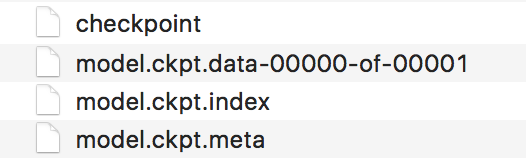
\includegraphics[width=6cm]{imgs/tf_model_checkpoints.png}
\end{figure}

\item Voc� pode utilizar esses arquivos para infer�ncia, no entanto, n�o s�o adequados para o ambiente de produ��o.
\end{itemize}

\vspace{1cm}
\tiny{Paper: \href{https://www.freecodecamp.org/news/how-to-deploy-an-object-detection-model-with-tensorflow-serving-d6436e65d1d9/}{How to deploy an Object Detection Model with TensorFlow serving}}
\end{frame}

%%%%%%%%%%%%%%%%%%%%%%%%%%%%%%%%%%%%%%%%%%%%%%%%%%%%%%%%%%%%%%%%%%%%%%%%%%%%%%%%%%%%%%%%%%%%%%%%%%%%%%%%%%%%%%%%

\begin{frame}[fragile]{TF Serving}
\begin{itemize}
\item Podemos converter o modelo para um {\it frozen graph}, que cont�m a arquitetura do modelo e os pesos em um �nico arquivo.
\item Para isso, utilize o script {\it export.py} presente no \href{https://github.com/freds0/fault_detection_power_transmission_lines}{c�digo de treinamento}:
\end{itemize}
\begin{verbatim}
$ python export.py \
    --config_file=configs/parameters.yaml \
    --pipeline_config_file=pipeline_file.config \
    --checkpoint_dir=checkpoints_folder \
    --output_export_dir=exported_checkpoints
\end{verbatim}

\vspace{1cm}
\tiny{C�digo: \href{https://github.com/freds0/fault_detection_power_transmission_lines}{https://github.com/freds0/fault\_detection\_power\_transmission\_lines}}
\end{frame}


%%%%%%%%%%%%%%%%%%%%%%%%%%%%%%%%%%%%%%%%%%%%%%%%%%%%%%%%%%%%%%%%%%%%%%%%%%%%%%%%%%%%%%%%%%%%%%%%%%%%%%%%%%%%%%%%%
\section{gRPC}
%%%%%%%%%%%%%%%%%%%%%%%%%%%%%%%%%%%%%%%%%%%%%%%%%%%%%%%%%%%%%%%%%%%%%%%%%%%%%%%%%%%%%%%%%%%%%%%%%%%%%%%%%%%%%%%%

\begin{frame}{gRPC}
\begin{itemize}
\item Ap�s converter os checkpoints, podemos "servir" o modelo utilizando o TF Serving.
\item O TF Serving utiliza o protocolo gRPC, desenvolvivo pelo Google.
\item O gRPC permite que um cliente execute uma fun��o em um servidor remoto
\end{itemize}

\vspace{1cm}
\tiny{Fonte: \href{https://grpc.io/}{gRPC - A high performance, open source universal RPC framework}}
\end{frame}


%%%%%%%%%%%%%%%%%%%%%%%%%%%%%%%%%%%%%%%%%%%%%%%%%%%%%%%%%%%%%%%%%%%%%%%%%%%%%%%%%%%%%%%%%%%%%%%%%%%%%%%%%%%%%%%%

\begin{frame}{gRPC}
\begin{figure}[h]
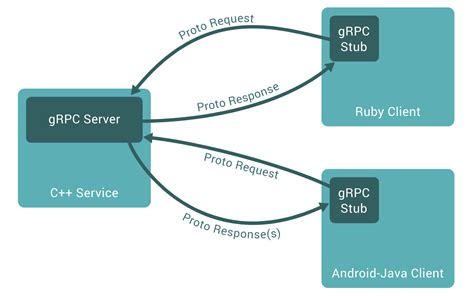
\includegraphics[width=8cm]{imgs/grpc_architecture.jpg}
\end{figure}

\end{frame}

%%%%%%%%%%%%%%%%%%%%%%%%%%%%%%%%%%%%%%%%%%%%%%%%%%%%%%%%%%%%%%%%%%%%%%%%%%%%%%%%%%%%%%%%%%%%%%%%%%%%%%%%%%%%%%%%

\begin{frame}{gRPC}
\begin{itemize}
\item O gRPC utiliza {\it Protocol Buffers} para serializar os dados.
\item Dessa forma, os dados ficam menores quando comparados com JSON e XML.
\item Assim, � necess�rio definir uma interface que utilize esse protocolo.
\end{itemize}

\vspace{1cm}
\tiny{Fonte: \href{https://grpc.io/}{gRPC - A high performance, open source universal RPC framework}}
\end{frame}

%%%%%%%%%%%%%%%%%%%%%%%%%%%%%%%%%%%%%%%%%%%%%%%%%%%%%%%%%%%%%%%%%%%%%%%%%%%%%%%%%%%%%%%%%%%%%%%%%%%%%%%%%%%%%%%%%
\section{Aplica��o}
%%%%%%%%%%%%%%%%%%%%%%%%%%%%%%%%%%%%%%%%%%%%%%%%%%%%%%%%%%%%%%%%%%%%%%%%%%%%%%%%%%%%%%%%%%%%%%%%%%%%%%%%%%%%%%%%

\begin{frame}{Aplica��o}
\begin{itemize}
\item A aplica��o � dividida em {\it backend} e {\it frontend}.
\item No {\it backend} tem-se uma aplica��o TF-Serving aguardando chamadas na porta 5000.
\item No {\it frontend} tem-se uma aplica��o Web rodando na porta 8000.
\end{itemize}

\vspace{1cm}
\tiny{C�digo: \href{https://github.com/freds0/flask_fault_detection_power_transmission_lines}{https://github.com/freds0/flask\_fault\_detection\_power\_transmission\_lines}}
\end{frame}


%%%%%%%%%%%%%%%%%%%%%%%%%%%%%%%%%%%%%%%%%%%%%%%%%%%%%%%%%%%%%%%%%%%%%%%%%%%%%%%%%%%%%%%%%%%%%%%%%%%%%%%%%%%%%%%%

\begin{frame}{Referencias}
\begin{itemize}
\item Documenta��o Oficial Tensorflow
  \begin{itemize}
  \item \url{https://www.tensorflow.org/tfx/guide/serving2}
  \end{itemize}
\item How to deploy an Object Detection Model with TensorFlow serving
  \begin{itemize}
  \item \url{https://www.freecodecamp.org/news/how-to-deploy-an-object-detection-model-with-tensorflow-serving-d6436e65d1d9/}
  \end{itemize}  
\end{itemize}
\end{frame}

%%%%%%%%%%%%%%%%%%%%%%%%%%%%%%%%%%%%%%%%%%%%%%%%%%%%%%%%%%%%%%%%%%%%%%%%%%%%%%%%%%%%%%%%%%%%%%%%%%%%%%%%%%%%%%%%

\begin{frame}[plain]
  \titlepage
\end{frame}


\end{document}
